\subsubsection{Electrical System}

\paragraph{Control Units} \ \\
\vspace{-0.5cm}

\vspace{-\baselineskip}
\begin{enumerate}[label=(\roman*), leftmargin=0pt, itemindent=20pt]
    \setlength{\itemsep}{0pt}
    \item \textbf{Topside Control Unit}

    \noindent\ignorespaces The Topside unit is where the pilot and the main program function. Several components are used to make up the topside control unit, which are shown in table \ref{tab:rov_components}.

    \begin{longtblr}[
        caption = {ROV Station Components and Functions},
        label = {tab:rov_components},
        entry = {Table \thetable}
      ]{
        width = 0.5\textwidth,
        colspec = {| Q[wd=0.1\textwidth, m] | X[m] |},
        hline{1,Z} = {solid},
        hline{2-Y} = {solid},
        rows = {font=\tiny},
        row{1} = {font=\bfseries\tiny},
        rowhead = 0
      }
    {Station Component} & {Function} \\
    {Logitech G Extreme 3D Pro Joystick} & {Used for controlling the ROV's motion.} \\
    {Laptop} & {Used for displaying all information received from the underwater unit.} \\
    {Power Source} & {Provides 48V operating voltage and a current maximum rating of 30A.} \\
    {Compressor} & {Used for supplying compressed air to the ROV's manipulator.} \\
    {Monitor} & {Used for displaying video feeds from the ROV} \\
    {Router} & {Used for establishing a wired connection between the ROV and the topside control unit.} \\
    {Anderson connector} & {A type of electrical connector used for connection power to the ROV} \\
    \end{longtblr}

    For efficient control and communication between the topside control unit and the ROV, the components found in Table \ref{tab:vehicle_components} are used in the vehicle.

    \begin{longtblr}[
        caption = {Vehicle Components and Functions},
        label = {tab:vehicle_components},
        entry = {Table \thetable}
      ]{
        width = 0.5\textwidth,
        colspec = {| Q[wd=0.1\textwidth, m] | X[m] |},
        hline{1,Z} = {solid},
        hline{2-Y} = {solid},
        rows = {font=\tiny},
        row{1} = {font=\bfseries\tiny},
        rowhead = 0
      }
    {Vehicle \newline Component} & {Function} \\
    {T200 Thrusters with ESC} & {Thrusters used for controlling the ROV's motion, including the Electronic Speed Controller (ESC)} \\
    {48V to 12V DC-DC Converters} & {Converts the operating 48V to 12V} \\
    {Raspberry pi 5} & {A powerful microcontroller used for processing and controlling the ROV} \\
    {STM32} & {A microcontroller board used for controlling various functions of the ROV} \\
    {1080p USB wide-angle Cameras} & {Providing high quality footage for tasks like navigation and 3D modelling.} \\
    {720p USB camera} & {Providing footage from sides of the vehicle.} \\
    {Zed 2i stereo camera} & {Depth camera that captures 3D images, generates depth maps} \\
    {W5500 Ethernet module} & {For real-time system monitoring and debugging} \\
    {CAN bus module} & {Ensures efficient and reliable communication between nodes} \\
    \end{longtblr}
    
    \item \textbf{Sensors}
    
    To provide the necessary data to control the ROV, different sensors are used, each for the different parameters. The sensors used can be found in the following table \ref{tab:sensors}.

    \begin{longtblr}[
        caption = {ROV Sensors and Functions},
        label = {tab:sensors},
        entry = {Table \thetable}
      ]{
        width = 0.5\textwidth,
        colspec = {| Q[wd=0.1\textwidth, m] | X[m] |},
        hline{1,Z} = {solid},
        hline{2-Y} = {solid},
        rows = {font=\tiny},
        row{1} = {font=\bfseries\tiny},
        rowhead = 0
      }
    {Sensor} & {Function} \\
    {Custom depth sensor (MS5837)} & {Measuring underwater pressure and depth level of the vehicle} \\
    {Arduino Nano RP2040 IMU} & {Measuring the angular velocity and linear acceleration of the vehicle} \\
    {Voltage \& Current Sensors (ACS712)} & {Track power consumption} \\
    \end{longtblr}

    \textbf{Implementation of a Custom-Designed Depth Sensor}

    A custom-designed depth sensor was introduced to replace the previously existing board. The new sensor delivered greater accuracy, real-time measurements, and supported a wider range of connectivity options. This upgrade significantly improved system performance and reliability, ensuring precise and efficient depth measurement.

    \item \textbf{Underwater Control Unit}
    
    The vehicle components are all mounted on 2 thoroughly designed PCBs for maximum efficiency and low space consumption, connecting all the microcontrollers and the sensors inside the ROV.
    \item \textbf{System Integration}
    
    The ROV's electrical system is interconnected through a structured communication framework. At the top side, the joystick sends control signals to the laptop, which transmits them to the router and then down the tether via an Ethernet cable. On the ROV side, an Ethernet switch distributes the signals, directing one output to the Raspberry Pi 5 (the primary controller) and another to the W5500 Ethernet module.
    
    \vspace{-0.2cm}
    \hspace{10pt} The system is designed as an integrated network of three modular subsystems. The Power Subsystem houses Electronic Speed Controllers (ESCs) and an STM32 microcontroller. The Raspberry Pi 5 sends control signals to the STM32 board, which then controls the seven ESCs connected to their respective T200 thrusters. Additionally, the STM32 microcontroller continuously collects real-time power consumption data of the thrusters and power converters, including current and voltage readings from the ACS712 current sensor, and transmits it to Raspberry Pi 5 via the CAN bus module for monitoring and analysis. 

    \vspace{-0.2cm}
    \hspace{10pt} The second subsystem is the Sensor System which includes the depth sensor and an Arduino Nano RP2040 for the IMU readings, both of which are connected to an STM32 microcontroller that handles data acquisition. STM32 processes the sensor data and sends it to Raspberry Pi 5 via the CAN bus protocol, ensuring timely and reliable data transmission. Finally, the Debugging subsystem which consists of an Ethernet module connected to an STM32 microcontroller, interfaced with the network switch via an Ethernet cable. Through CAN bus integration, the Ethernet module communicates with the other subsystems, enables real-time system debugging, allowing for troubleshooting of the entire system remotely. It also provides fault control, monitoring and managing any failures that may occur within the Power PCB or Sensor subsystem.
    
    \vspace{-0.2cm}
    \hspace{10pt} Finally, the camera’s video feed is processed by the Raspberry Pi 5, transmitted back to the topside through the tether, and displayed on the GUI on the laptop. Additionally, all other sensor data, including depth measurements, current and voltage values from the Power PCB, and IMU from the Arduino Nano RP2040, are collected by the STM32 microcontrollers and sent to the Raspberry Pi 5 via CAN bus. The Raspberry Pi then transmits this information via ROS to the topside control station, where it is displayed on the GUI for real-time monitoring.
\end{enumerate}

\vspace{-1cm}
\paragraph{Electric Power} \ \\
\vspace{-0.5cm}

The provided power is 48 V and with a maximum of 30 A. This power needs to be converted and well distributed to suit our needs in the ROV, as powering the thrusters, ESCs, vision system, development boards, and other peripherals.

\vspace{-0.5\baselineskip}
\begin{enumerate}[label=(\roman*), leftmargin=0pt, itemindent=20pt]
    \setlength{\itemsep}{0pt}
    \item \textbf{Power Conversion System}
    
    The 48-Volt supply voltage is converted into 12 V using five different DC-DC Step down converters. Four of the converters provide a current of 30 Amps, and the fifth one provides 10 Amps. The total current is then distributed to the thrusters and the power unit PCB to supply power to the other boards inside the canister. In addition, there are Four 12V-to-5V step-down (buck) converters inside the power unit PCB, two of them provide 5 Amps for the Raspberry Pi board. The other twp provide 3 amps, one of them supplying STM32 microcontrollers and the CAN bus modules in the power PCB while the other supply the sensors and other indicators. Details of power distribution can be seen in Table \ref{tab:power_calculation}.

    \begin{table}[hb!]
        \centering
        \begin{adjustbox}{max width=0.9\columnwidth}
        \begin{tabular}{@{} l *{5}{c} @{}}
          \toprule
          \textbf{Component} & \textbf{Quantity} & \textbf{Voltage (V)} & \textbf{Current (A)} & \textbf{Power Per Unit (W)} & \textbf{Total Power (W)} \\
          \midrule
          T200 Thruster            & 7 & 12   & 12     & 144    & 1008   \\
          Basic ESC                & 7 & 12   & 0.15   & 1.8    & 12.6   \\
          Raspberry Pi 5           & 1 & 5    & 5      & 25     & 25     \\
          STM32                    & 4 & 3.3  & 0.125  & 0.4125 & 1.65   \\
          MCP2515 CAN Bus Module   & 5 & 5    & 0.1    & 0.5    & 2.5    \\
          W5500 Ethernet Module    & 1 & 5    & 0.13   & 0.65   & 0.65   \\
          Arduino Nano RP2040      & 1 & 5    & 0.45   & 2.25   & 2.25   \\
          720p USB Camera          & 3 & 5    & 0.2    & 1      & 3      \\
          1080p USB camera         & 2 & 5    & 0.275  & 1.375  & 2.75   \\
          MS5837 Depth Sensor      & 1 & 5    & 0.002  & 0.01   & 0.01   \\
          ZED 2i stereo camera     & 1 & 5    & 0.5    & 2.5    & 2.5    \\
          \midrule
         \multicolumn{5}{l}{\textbf{Total}} & \textbf{1060.91} \\
          \bottomrule
        \end{tabular}
        \end{adjustbox}
    \caption{Power Calculation for the ROV.}
    \label{tab:power_calculation}
    \end{table}

    Total Current Drawn at 48V: \( 1060.9 / 48 = 21.10 \, \text{A} \), Applying Safety Factor: \( 1.3 \times 21.10 = 28.73 \, \text{A} \)
    \setlength{\parskip}{0pt}

    Required Fuse = 30A

    \item \textbf{Power Unit}
    
    As mentioned above, two PCB containing three subsystems were designed specifically for the power conversion system inside the ROV.
\end{enumerate}

\vspace{-0.8cm}
\paragraph{Tether} \ \\
\vspace{-0.5cm}

The tether is made of Polyethylene Terephthalate (PET) light weight 15mm expandable cable sleeve which provides protection for the cables inside (Figure \ref{fig:tether}). Tether length is 25 meters long and consists of two 16mm2 cables made from Aluminum and PVC jacket material. CAT6e for ethernet communication. The 2 pneumatic hose supply is also included in the tether, one as an inlet and the other as an outlet.

\begin{figure}[h!]
    \centering
    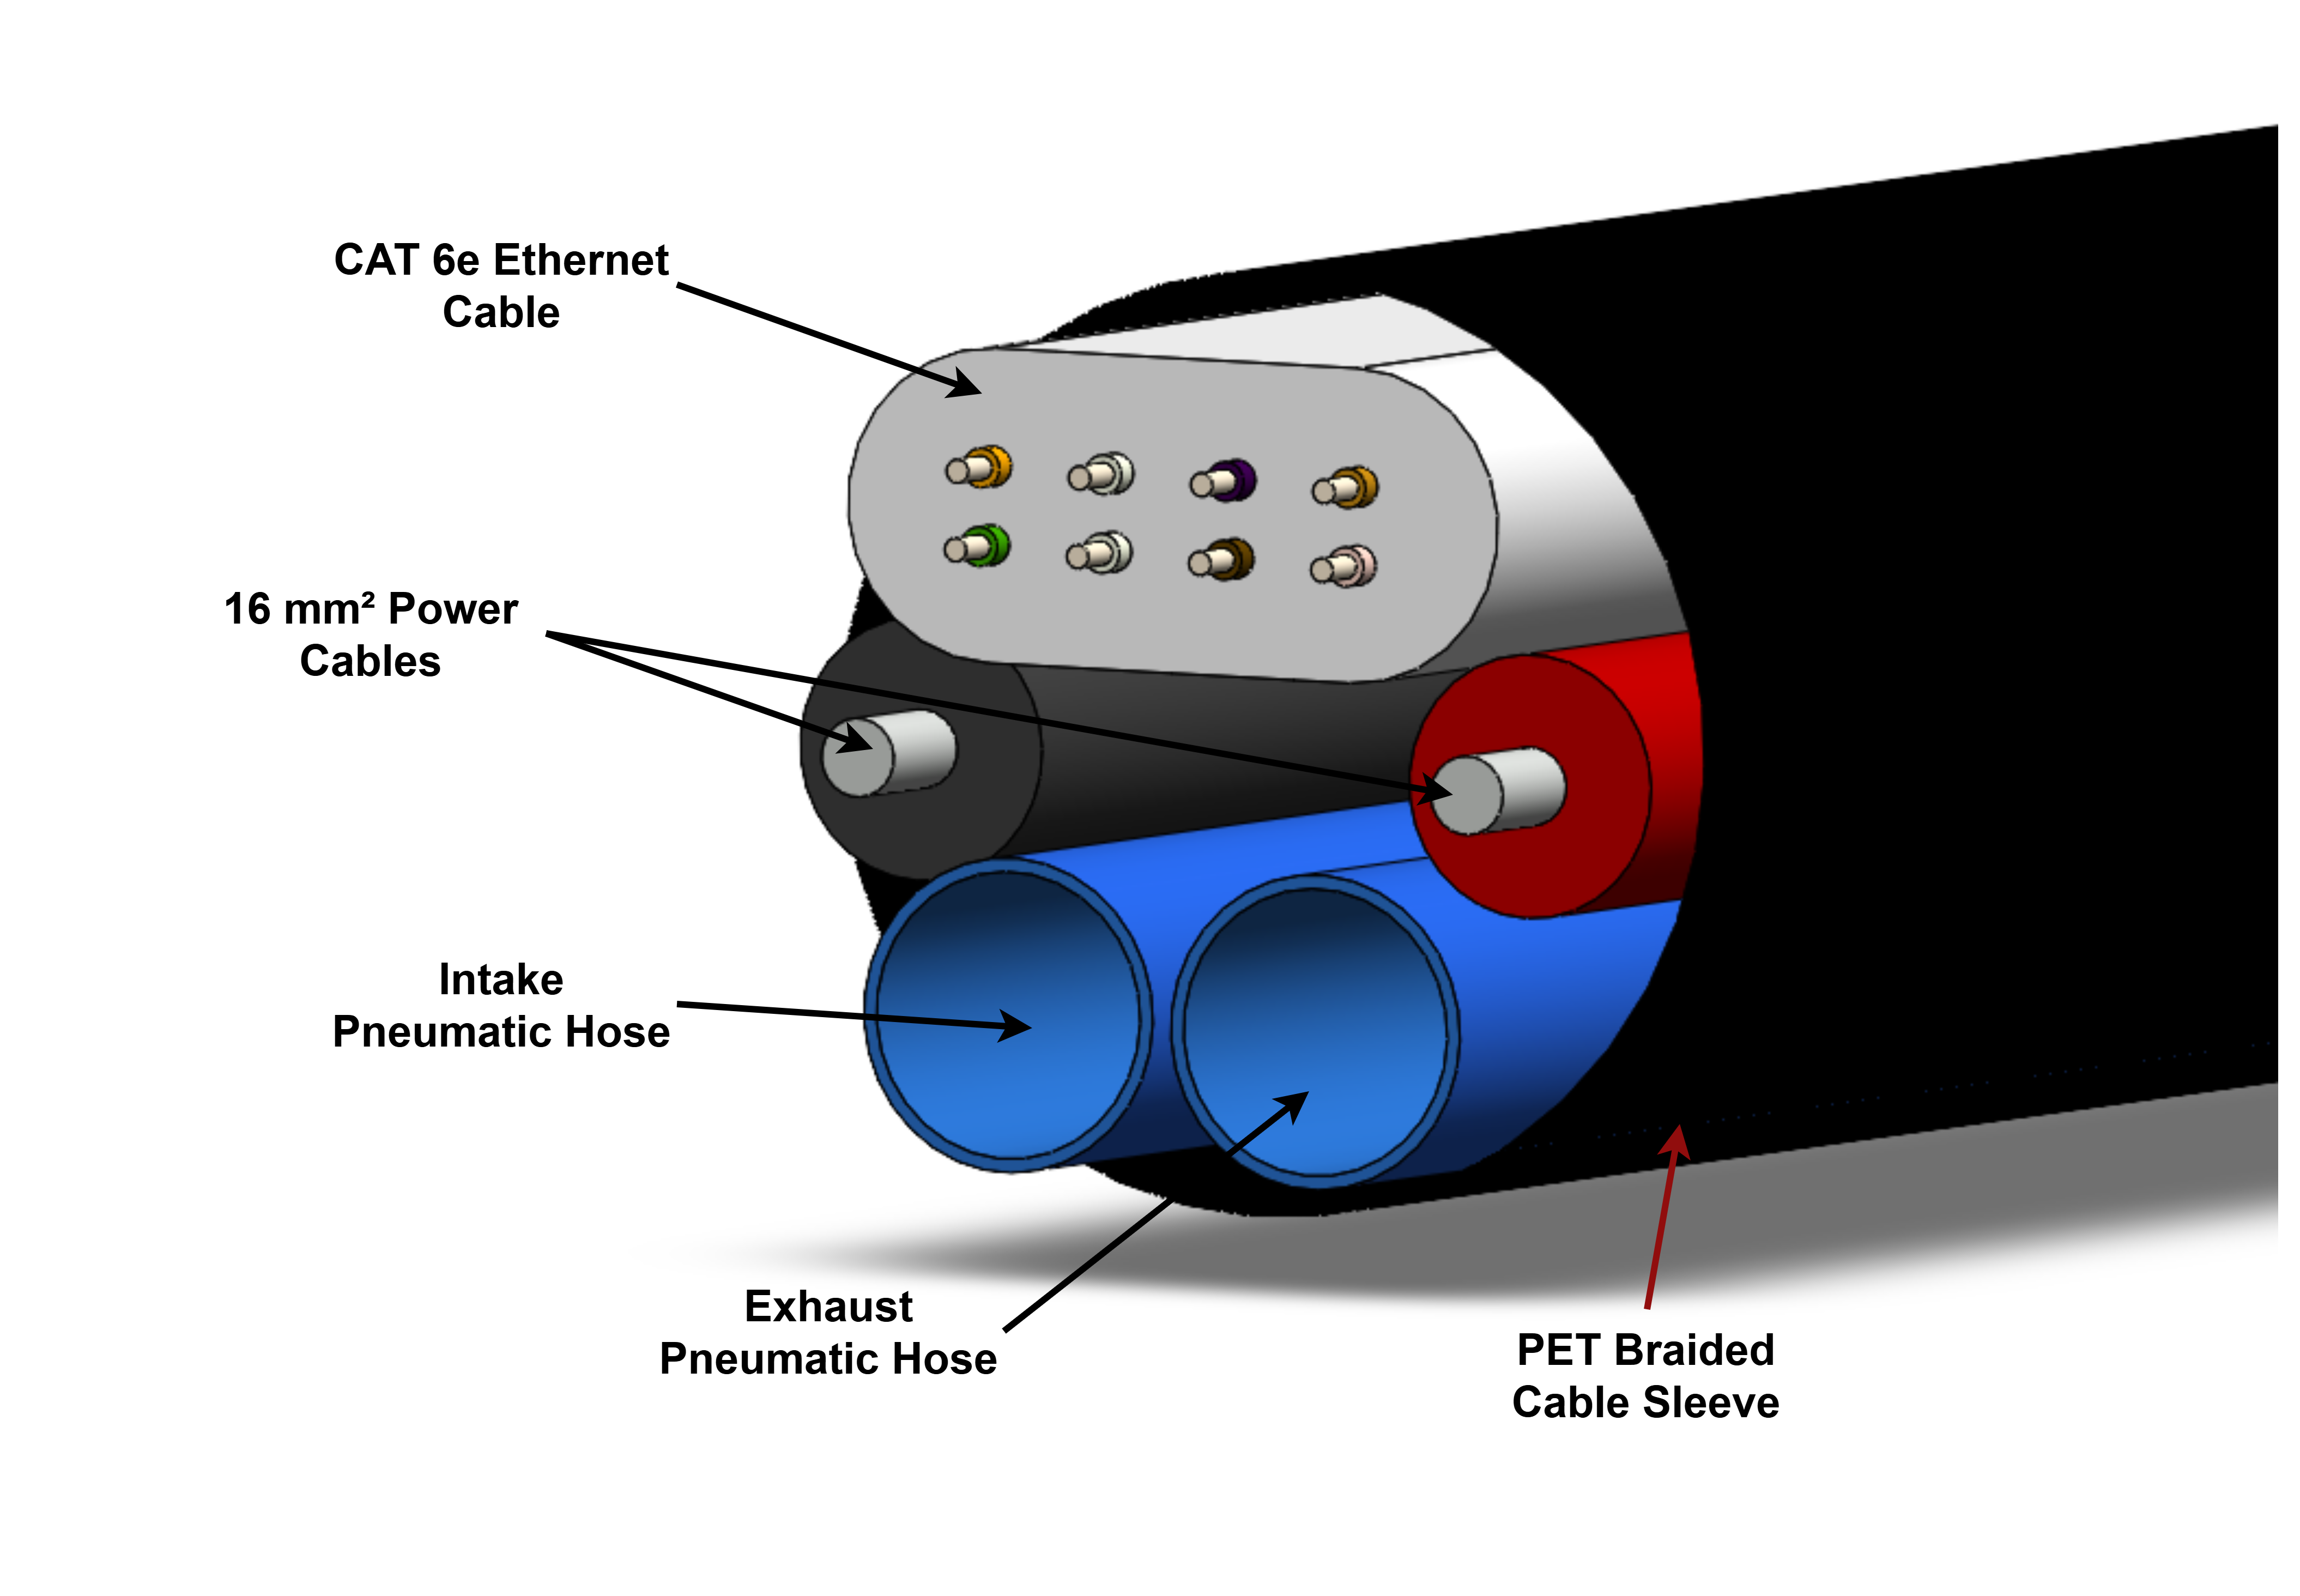
\includegraphics[width=0.8\columnwidth]{Sections/2Design Rationale/images/Tether.png}
    \caption{Tether Cross Section.}
    \label{fig:tether}
\end{figure}